Per assicurarsi che i requisiti individuati nell'\AdR \ vengano soddisfatti, è necessario implementare dei test che ne verifichino l'effettiva implementazione.

\subsubsection{Test di sistema previsti}

\begin{tabularx}{\textwidth}{cXc}
	
	\rowcolor{greySWEight}
	
	\rowcolor{greySWEight}
	\textcolor{white}{\textbf{Codice}} & 
	\textcolor{white}{\textbf{Descrizione}} &
	\textcolor{white}{\textbf{Stato}} \\
	
	\textbf{TS001} & Verifica che un utente non autenticato possa autenticarsi nel sistema & \textcolor{ForestGreen}{Superato} \\
	\textbf{TS002} & Verifica che un utente non autenticato possa registrarsi & \textcolor{ForestGreen}{Superato} \\
	\textbf{TS003} & Verifica che un insegnante possa inserire un nuovo esericizio di analisi grammaticale & \textcolor{ForestGreen}{Superato} \\
	\textbf{TS004} & Verifica che un insegnante possa usufruire del servizio di
	correzione automatica da parte della libreria di Pos-Tagging & \textcolor{ForestGreen}{Superato} \\
	\textbf{TS005} & Un allievo può visualizzare i propri progressi & Non Implementato \\
	\textbf{TS006} & Un allievo può visualizzare i propri traguardi & Non Implementato \\
	\textbf{TS007} & Verifica che un allievo possa visualizzare le sue valutazioni & Non Implementato \\
	\textbf{TS008} & Verifica che un allievo possa inserire un insegnante come preferito & Non Implementato \\
	\textbf{TS009} & Verifica che un allievo possa inserire una frase libera da svolgere autonomamente per poi ricevere
	una valutazione automatica & \textcolor{ForestGreen}{Superato} \\
	\textbf{TS010} & Verifica che un allievo possa visualizzare l’elenco degli
	esercizi assegnati dall’insegnante & \textcolor{ForestGreen}{Superato} \\
	\textbf{TS011} & Verifica che un allievo possa svolgere un esercizio di analisi grammaticale & \textcolor{ForestGreen}{Superato} \\
	\textbf{TS012} & Verifica che uno sviluppatore possa visualizzare l’elenco delle frasi registrate & Non Implementato \\
	\textbf{TS013} & Verifica che uno sviluppatore possa scaricare i dati & Non Implementato \\
	\textbf{TS014} & Verifica che un amministratore possa eliminare un'utenza dal sistema & \textcolor{ForestGreen}{Superato} \\
	\textbf{TS015} & Verifica che un amministratore possa visualizzare le richieste di attivazione degli sviluppatori & \textcolor{ForestGreen}{Superato} \\
	\textbf{TS016} & Verifica che un amministratore possa rifiutare un'utenza di tipo sviluppatore & \textcolor{ForestGreen}{Superato} \\
	
	\rowcolor{white}
	\caption{Test di sistema}
	\label{tab:tabellatestsistema}
\end{tabularx}

\begin{figure}[H]
	\centering
	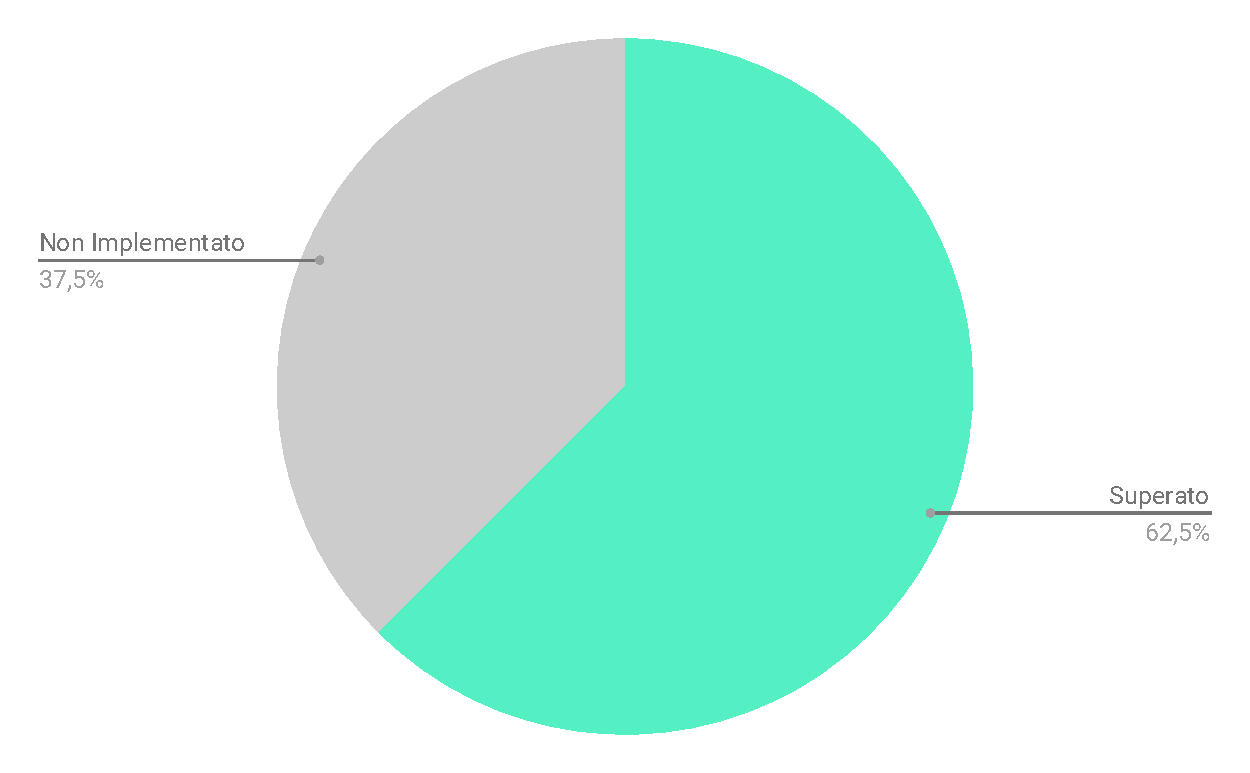
\includegraphics[width=0.7\linewidth]{sez/test/img/statoTestSistema.pdf}
	\caption{Riepilogo stato test di sistema}
\end{figure}

\subsubsection{Tracciamento Test di sistema - Requisiti}

\begin{tabularx}{\textwidth}{cX}
	
	\rowcolor{greySWEight}
	
	\rowcolor{greySWEight}
	\textcolor{white}{\textbf{Test}} & 
	\textcolor{white}{\textbf{Requisiti}} \\
	
	TS001 & R-1F001 \\
	TS002 & R-1F004 \\
	TS003 & R-1F013 \\
	TS004 & R-1F015 \\
	TS005 & R-1F030 \\
	TS006 & R-1F031 \\
	TS007 & R-1F032 \\
	TS008 & R-1F034 \\
	TS009 & R-1F038 \\
	TS010 & R-1F036 \\
	TS011 & R-1F040 \\
	TS012 & R-1F053 \\
	TS013 & R-1F054 \\
	TS014 & R-1F064 \\
	TS015 & R-1F065 \\
	TS016 & R-1F067 \\
	
	\rowcolor{white}
	\caption{Tracciamento test di sistema - requisiti}
	\label{tab:tracciamentotestsistema}
\end{tabularx}
